\documentclass[12pt]{article}

\usepackage{sbc-template}

\usepackage{graphicx,url}

\usepackage[brazil]{babel}   
%\usepackage[latin1]{inputenc}  
\usepackage[utf8]{inputenc}  
% UTF-8 encoding is recommended by ShareLaTex

\usepackage{listings}
     

\title{Paralelismo de dados usando \textit{PThreads} e \textit{OpenMP} para \textit{Covariance} do PolyBench/C 3.2}

\author{Alessandra H. Iriguti\inst{1}}

\address{Departamento de Informática -- Universidade Estadual de Maringá (UEM)\\
  Maringá -- PR -- Brazil
  \email{alehairi@gmail.com}
  \email{ra88741@uem.br}
}

\begin{document} 

\maketitle

\begin{abstract}
One of the techniques to take advantage of multiprocessors is data parallelism. It generates the race hazard, because it is shared memory and, in order to solve it, synchronization is used in critical section. In the end, it is expected to obtain good speedup, that is the sequential time divided by the parallel time for a determined number of threads. The algorithm to be parallelized is the PolyBench/C 3.2's covariance using PThreads and OpenMP interfaces. It was run eleven times for each combination of parameters (algorithm type and number of threads) on a computer with eight Intel Xeon @2.00 GHz physical processors. A good speedup was not achieved. The hardware analysis with PAPI indicates that the main reason for the low speedup was synchronization and inefficient implementation of the parallel codes.
\end{abstract}
     
\begin{resumo} 
Uma das técnicas de aproveitar multiprocessadores é o paralelismo de dados. Isso gera o problema de condição de corrida, pois a memória é compartilhada, e, para solucioná-la, utiliza-se sincronização na região crítica. No fim, espera-se obter um bom fator de aceleração que representa a fração do tempo sequencial sobre o paralelo para determinada quantidade de \textit{threads}. O algoritmo a ser paralelizado é o \textit{covariance} do PolyBench/C 3.2 e foram utilizadas as interfaces \textit{PThreads} e \textit{OpenMP}. Foram feitas onze execuções para cada combinação de parâmetros (tipo do algoritmo e número de \textit{threads}) em uma máquina com oito processadores físicos Intel Xeon @2.00 GHz. Não foi alcançado um bom \textit{speedup}. A análise do \textit{hardware} com o PAPI indicam que o fator impactante ao baixo \textit{speedup} foram a sincronização e uma implementação ineficiente dos códigos paralelos.
\end{resumo}


\section{Fundamentação}

O crescimento da necessidade de resolver problemas cada vez maiores exigiram evoluções nas arquiteturas dos computadores. Por exemplo, mais de um processador (ou núcleo de processador) nas máquinas. Apenas isso, porém, não era suficiente, uma vez que, neste caso (de computadores multiprocessadores), não era interessante que uma CPU ficasse ociosa, enquanto outra estava sendo totalmente utilizada. Em outras palavras, a evolução dos \textit{hardwares}, como processadores \textit{multicore}, a fim de melhorar o poder computacional, exige o surgimento de novas estratégias de programação que façam um uso proveitoso e eficaz dos multiprocessadores. Uma dessas técnicas é o paralelismo de dados.

\subsection{Paralelismo de dados}

O paralelismo de dados é uma técnica de programação que divide uma grande quantidade de dados em partes menores que podem ser computadas em paralelo. Em seguida, essas partes menores são recombinadas a um único conjunto. Cada tarefa executa uma mesma série de cálculos sobre diferentes dados. Dessa forma, é possível usar melhor do potencial dos processadores.

No problema de soma de dois vetores, por exemplo. Um algoritmo sem paralelização irá computar as instruções dentro de todos os \textit{for} de maneira sequencial. Existem diversas maneiras de se paralelizar. 

A abordagem adotada é a SMP (\textit{Symetric MultiProcessors}). Nela, o acesso à memória é compartilhada, em que os processadores acessam a mesma memória. Em problemas mais complexos, onde ocorrem leituras e escritas em um mesmo local de memória ou onde a computação de um dado depende do resultado de outro, deve haver um controle sobre os dados para que os processadores produzam o resultado correto.

\subsection{Condições de corrida e sincronização}

A condição de corrida é uma situação que ocorre quando há regiões críticas. Uma região crítica é uma porção de código que realiza a leitura e escrita na mesma posição de memória e em que o tempo em que ocorre a leitura ou escrita das \textit{threads} (fluxos de execução de instruções que podem ser escalonados pelo sistema operacional) podem influenciar para uma computação equivocada. 

Por exemplo, um algoritmo para contar quantos números pares aparecem em uma matriz. Possivelmente, haverá uma variável \textit{counter} para representar a quantidade de números pares. Em algum momento do código, depois de verificado e confirmado um número par, deverá haver um incremento na variável \textit{counter}. Primeiramente, ocorre a leitura do valor contido em \textit{counter} para então ser somado o valor 1 e, por fim, escrever o novo valor em \textit{counter}. Se há duas \textit{threads} computando essa tarefa, pode ocorrer condição de corrida. Em uma iteração em que as duas \textit{threads} encontram pares, a \textit{thread} T1 lê o valor de \textit{counter}, suponha que seja 3. Em seguida, a \textit{thread} T1 incrementa o valor de \textit{counter} para 4 e, no mesmo momento, a \textit{thread} T2 lê \textit{counter}, porém, como T1 ainda não escreveu, T2 leu 3. A T1 escreverá 4 em \textit{counter} e, depois, T2 também escreverá 4. No fim dessa iteração, \textit{counter} deveria valer 5, todavia, pode não ocorrer, como no caso descrito acima.

Há diversas soluções para esse problema. Uma solução é a  sincronização. A sincronização é o gerenciamento adequado de várias linhas de execução ou processos concorrentes que acessam a mesma região crítica. Por exemplo, o uso de \textit{locks}. Um \textit{lock} delimita as regiões críticas e faz com que apenas uma \textit{thread} execute a região crítica por vez. Isso é conhecido como exclusão mútua (ou pelo acrônimo \textit{mutex} para \textit{mutual exclusion}). Isto é, uma técnica usada em programação concorrente para evitar que dois processos ou \textit{threads} tenham acesso simultaneamente a uma seção crítica. Outro exemplo é o uso de barreiras. Uma barreira impede que uma \textit{thread} continue a sua execução a partir da barreira enquanto as outras \textit{threads} não alcançaram a barreira. A partir do momento que todas as \textit{threads} chegaram na barreira, a execução a partir dela é liberado.

\subsection{Fator de aceleração} \label{sec:speedup}

Umas das métricas de desempenho em sistemas paralelos é o fator de aceleração, ou em inglês \textit{speedup}. O fator de aceleração relaciona é a relação do tempo do algoritmo sequencial sobre o tempo do algoritmo paralelo, para um mesmo problema e de mesmo tamanho. Formalmente, o fator de aceleração $S$ é dado por:

$$ S\left(p\right)=\frac{t_s}{t_p}
$$

Em que $t_s$ é o tempo da execução do algoritmo sequencial e, $t_p$, o tempo da execução do algoritmo paralelo para $p$ indica o número de processadores utilizados.

Diversos fatores podem limitar o aumento do \textit{speedup}, tais como períodos de ociosidade e comunicação entre processadores. Além disso, nem todo código é paralelizável.

Considerando que o tempo de comunicação entre os processadores seja desprezível, na computação ideal, quanto maior o número de processadores (ou \textit{threads}) utilizadas, maior seria o \textit{speedup}. Ou seja, seria uma função linear, uma bissetriz do primeiro quadrante. Por exemplo, suponha o $t_s=100$, na situação utópica, teríamos $S\left(2\right)=2$, $S\left(4\right)=4$, $S\left(8\right)=8$, $S\left(16\right)=16$ e assim sucessivamente. Todavia, não é o que acontece, já que existe um gasto de tempo (um \textit{overhead}) para a criação, destruição das \textit{threads}, além do \textit{overhead} que ocorre quando há sincronização.

\subsection{Interfaces de programação paralela}

Para a paralelização, inúmeros fabricantes de sistemas computacionais desenvolveram suas próprias bibliotecas. Estas eram focadas em características específicas de suas arquiteturas. Dessa forma, os códigos paralelizados não eram portáteis. A fim de solucionar isso, surgiram interfaces de programação (\textit{APIs}) paralelas que fossem eficientes e portáteis para qualquer arquitetura disponível. Duas delas são \textit{POSIX Threads} (ou simplesmente \textit{PThread}) e \textit{Open Multi-Processing Application Program Interface} (\textit{OpenMP}).

\subsubsection{\textit{PThreads}} \label{sec:pthreads}

\textit{PThreads} é uma interface de manipulação de \textit{threads} padronizada em 1995 pelo \textit{IEEE POSIX} 1003.1c \textit{standard}. São definidos como um conjunto de tipos e chamadas de procedimento de programação na linguagem C e estão presentes na biblioteca \textit{pthread.h}. Uma vantagem em utilizar \textit{PThreads} é que o custo de gerenciar \textit{threads} é menor que gerenciar processos. 

As subrotinas presentes em \textit{PThreads}, podem ser sintetizadas em quatro grupos: 

\begin{enumerate}
	\item Gerenciamento de \textit{Threads}: funções de criação, de destruição, de junção de \textit{threads}, entre outras;
	\item Exclusão mútua (\textit{mutex}): rotinas que lidam com sincronização. Criação, inicialização e destruição de \textit{mutexes}, \textit{locking} e \textit{unlocking}, entre outros;
	\item Variáveis condicionais: rotinas que abordam comunicações entre \textit{threads} que compartilham um \textit{mutex}, com base nas condições especificadas pelo programador. Criar, destruir, aguardar e assinalar de acordo com valores das variáveis especificadas; e
	\item Sincronização: rotinas que gerenciam leitura e escrita com base em \textit{locks} e barreiras.
\end{enumerate}

\subsubsection{\textit{OpenMP}} \label{sec:omp}

\textit{OpenMP} é uma API com de paralelismo de programas em linguagens C, C++ e Fortran. Consiste em uma coleção de diretivas de compilação, variáveis de ambiente e de rotinas pertencentes à biblioteca \textit{omp.h}. Esse conjunto é usado pelo programador de maneira explícita o trecho do código a ser paralelizado. 

Toda diretiva é iniciada com \textit{\#pragma omp} e é aplicada em até uma declaração sucessora que deve ser um bloco estruturado. A seguir serão apresentadas apenas as construções relevantes para o propósito deste artigo.

A primeira construção a ser apresentada é a \textit{parallel} que inicia uma execução paralela. Para determinar o número de \textit{threads} a computarem o código delimitado pela primeira diretiva, basta usar com a variável \textit{num\_threads(p)}, em que $p$ é a quantidade de \textit{threads}. Ou seja, para iniciar uma execução paralela com $p$ \textit{threads}, utiliza-se a diretiva \textit{\#pragma omp parallel num\_threads(p)}.

Outra construção é para a forma canônica de \textit{loops}. Para ela, utiliza-se a diretiva \textit{for} que deve ser seguida de apenas uma instrução, que no caso é um \textit{for}. Esta pode ser utilizada juntamente à construção \textit{simd}. Ela indica que múltiplas iterações do laço de repetição podem ser executadas de maneira concorrente usando instruções SIMD (\textit{Single Instructions Multiple Datas}). Se há mais de um \textit{for} associado à construção \textit{simd}, então as iterações de todos esses \textit{for} são transformadas em apenas uma iteração maior, onde serão executadas instruções SIMD. A construção final ficaria \textit{\#pragma omp for simd}.

Vale ressaltar que o \textit{\#pragma omp for simd} implementa implicitamente uma barreira. Isso significa que o segundo \textit{for} só é iniciado quando todas as \textit{threads} terminarem o primeiro \textit{for}, e assim sucessivamente.

\section{Proposta}

O objetivo é verificar o \textit{speedup}, tanto utilizando  \textit{PThreads} quanto utilizando \textit{OpenMP}. Para isso, foram implementados para o \textit{benchmark Covariance} duas versões paralelas, uma para cada interface.

\subsection{\textit{Covariance}}

O programa \textit{Covariance} foi retirado da coleção de \textit{benchmarks} chamada \textit{Polyhedral Benchmark suite}, ou, simplesmente, PolyBench. A versão utilizada é o PolyBench/C 3.2. \textit{Covariance} calcula a covariância, uma medida estatística que mostra o quão duas variáveis estão linearmente relacionadas. Como entrada, recebe uma matriz \textit{data} de dimensões $N \times M$, que representa os $N$ pontos de dados com $M$ atributos. Após a computação, retorna uma matriz \textit{cov} simétrica $M \times M$, em que o $i,j$-ésimo elemento é a covariância entre $i$ e $j$. 

Matematicamente, covariância é definida como a média (\textit{mean}) dos produtos dos desvios para $i$ e $j$. Portanto temos:

$$ cov\left(i,j\right)=\frac{\sum_{k=0}^{N-1} \left(data\left(k,i\right)-mean\left(i\right)\right)\left(data\left(k,j\right)-mean\left(j\right)\right)}{N-1}
$$
Onde:
$$ mean\left(x\right)=\frac{\sum_{k=0}^{N-1} data\left(k,x\right)}{N}
$$

O código sequencial do PolyBench/C 3.2 para o cálculo da covariância segue abaixo:

{\scriptsize
\begin{lstlisting}
static void kernel_covariance(int m, int n, DATA_TYPE float_n) {

	int i, j, j1, j2;
	
	/* Determine mean of column vectors of input data matrix */
	for (j = 0; j < _PB_M; j++) {
		mean[j] = 0.0;
		for (i = 0; i < _PB_N; i++)
			mean[j] += data[i][j];
		mean[j] /= float_n;
	}
	
	/* Center the column vectors. */
	for (i = 0; i < _PB_N; i++)
		for (j = 0; j < _PB_M; j++)
			data[i][j] -= mean[j];
	
	/* Calculate the m * m covariance matrix. */
	for (j1 = 0; j1 < _PB_M; j1++)
		for (j2 = j1; j2 < _PB_M; j2++) {
			symmat[j1][j2] = 0.0;
			for (i = 0; i < _PB_N; i++)
				symmat[j1][j2] += data[i][j1] * data[i][j2];
			symmat[j2][j1] = symmat[j1][j2];
		}
	
}
\end{lstlisting}}

Em que a matriz \textit{data} representa o $data$ presente na fórmula matemática, assim como o vetor \textit{mean}. A matriz \textit{symmat} representa o $cov\left(i,j\right)$ da equação. Como pode ser observado, há três \textit{for} maiores, externos. Destes três, dois são duplos (dois \textit{for} aninhados) e um triplo. 

Paralelizando o código com \textit{PThreads}, obtem-se o seguinte código abaixo:

{\scriptsize
\begin{lstlisting}
void *covariance_pthread(void *argumentos) {
	int colunai, colunaf;
	int i, j, j1, j2;
	int n,m;
	
	struct args *a;
	a = (struct args *) argumentos;
	colunai = (int) a->colunai;
	colunaf = (int) a->colunaf;
	n = (int) a->n;
	m = (int) a->m;
	
	for (j = colunai; j < colunaf; j++) {
		mean[j] = 0.0;
		for (i = 0; i < _PB_N; i++) {
			mean[j] += data[i][j];
		}
		mean[j] /= float_n;
	}
	
	for (i = 0; i < _PB_N; i++) {
		for (j = colunai; j < colunaf; j++) {
			data[i][j] -= mean[j];
		}
	}
	
	pthread_barrier_wait (&barreira);
	for (j1 = colunai; j1 < colunaf; j1++){
		for (j2 = j1; j2 < _PB_M; j2++) {
			symmat[j1][j2] = 0.0;
			for (i = 0; i < _PB_N; i++) {
				symmat[j1][j2] += data[i][j1] * data[i][j2];
			}
			symmat[j2][j1] = symmat[j1][j2];
		}
	}
}
\end{lstlisting}}

A ideia utilizada para essa paralelização, foi dividir a mesma quantidade de colunas da matriz \textit{data} para cada \textit{thread}. Consequentemente, cada \textit{thread} ficaria responsável pela computação da mesma quantidade de linhas da matriz \textit{symmat}. Foi necessário o uso de uma barreira antes do \textit{for} tripo. Este usa resultados do segundo \textit{for} e, como diversas \textit{threads} computam seus resultados, é necessário uma barreira para aguardar a finalização dessa computação para continuar a execução e calcular o resultado final.

Por fim, paralelizando com \textit{OpenMP}, foram utilizadas as diretivas destacadas na seção \ref{sec:omp}.

{\scriptsize
\begin{lstlisting}
void covariance_openmp(int m, int n, int nt, DATA_TYPE float_n) {

	#pragma omp parallel num_threads(nt)
	{
		#pragma omp for simd
		for (int j = 0; j < _PB_M; j++) {
			mean[j] = 0.0;
			for (int i = 0; i < _PB_N; i++) {
				mean[j] += data[i][j];
			}
			mean[j] /= float_n;
		}
		
		#pragma omp for simd
		for (int i = 0; i < _PB_N; i++)
			for (int j = 0; j < _PB_M; j++)
				data[i][j] -= mean[j];
		
		#pragma omp for simd
		for (int j1 = 0; j1 < _PB_M; j1++)
			for (int j2 = j1; j2 < _PB_M; j2++) {
				symmat[j1][j2] = 0.0;
				for (int i = 0; i < _PB_N; i++) {
					symmat[j1][j2] += data[i][j1] * data[i][j2];
				}
				symmat[j2][j1] = symmat[j1][j2];
			}
	}
}
\end{lstlisting}}

A diretiva \textit{\#pragma omp parallel num\_threads($nt$)} cria $nt$ \textit{threads} para executarem paralelamente o código delimitado por essa diretiva. Essas \textit{threads} são só destruídas no fim, depois do término na execução do \textit{for} triplo. Outra diretiva utilizada foi o \textit{\#pragma omp for simd}, para possibilitar a execução em paralelo do \textit{for} que segue imediatamente tal diretiva. 

\section{Ambiente de execução}

A máquina utilizada para as execuções dos algoritmos possui 8 processadores físicos e Ubuntu 15.10 (GNU/Linux 4.2.0-22-generic) como sistema operacional. O processador é Intel(R) Xeon(R) CPU E5504 @2.00GHz, com arquitetura x86, 64-bits, Little Endian. Possui três níveis de cache, em que a L1 possui $32K$, a L2 possui $256K$ e a L3 $4096K$ e possui sete contadores de \textit{hardware}.

\subsection{Estratégias de execuções}

Para a coleta de resultados, foram adotadas algumas estratégias. Primeiramente, foi avaliado se o aumento do tamanho do problema influenciava no fator de aceleração, já que os tempos entre o sequencial e o paralelo apresentaria vantagem quando o tempo sequencial era consideravelmente alto (aproximadamente cinco minutos). Porém, após vários testes, conclui-se que o tamanho da entrada não influenciava no cálculo do \textit{speedup}. Dessa forma, foi selecionado o tamanho de $2048$. 

Para verificar a distância da forma ideal linear, foi calculado \textit{speedup} para $2$, $4$, $8$, $16$ e $32$ \textit{threads}. Isso foi feito para \textit{PThread} e \textit{OpenMP}. Além disso, para maior precisão de dados, foram realizadas onze execuções. Ou seja, foram executadas onze vezes o sequencial, onze vezes usando \textit{PThreads} para $4$, $8$, $16$ e $32$ \textit{threads} e onzes vezes usando \textit{OpenMP} para $4$, $8$, $16$ e $32$ \textit{threads}. Após as execuções, três tempos foram descartados: a da primeira execução, pois esta serve apenas para "aquecer" a \textit{cache}; a de maior tempo e a de menor tempo, para eliminar os tempos mais dispersos do conjunto. Em seguida, foi feito a média dos oito tempos restantes. Estes foram utilizados para calcular o fator de aceleração. Com esses dados, foi feito o gráfico de \textit{speedup} (Figura \ref{fig:speedup}).

Por fim, foi utilizado a ferramenta PAPI (\textit{Performance Application Programming Interface}) na versão $5.4.1.0$ para monitorar a relação entre o \textit{hardware} (o ambiente de execução) e o \textit{sofware} (o programa em questão). Com ele foram capturados os dados de número total de \textit{cache miss} nos três níveis: L1, L2 e L3; total de instruções ponto flutuante; total de ciclos e total de instruções. Foram recolhidos esses dados e feitas as médias desses valores para cada operação (sequencial, \textit{PThread} e \textit{OpenMP}).

\section{Resultados} \label{sec:resultados}

Na figura \ref{fig:speedup}, é possível observar o fator de aceleração para o algoritmo \textit{covariance}. A linha pontilhada de cor lilás se refere à situação ideal, quanto maior o número de \textit{threads} maior o \textit{speedup}. Porém o que ocorreu estão representadas nas linhas verde (\textit{PThread}) e azul claro (\textit{OpenMP}). A queda no crescimento dessas duas curvas já era esperado, devido a motivos já discutidos na seção \ref{sec:speedup}.

\begin{figure}[ht]
	\centering
	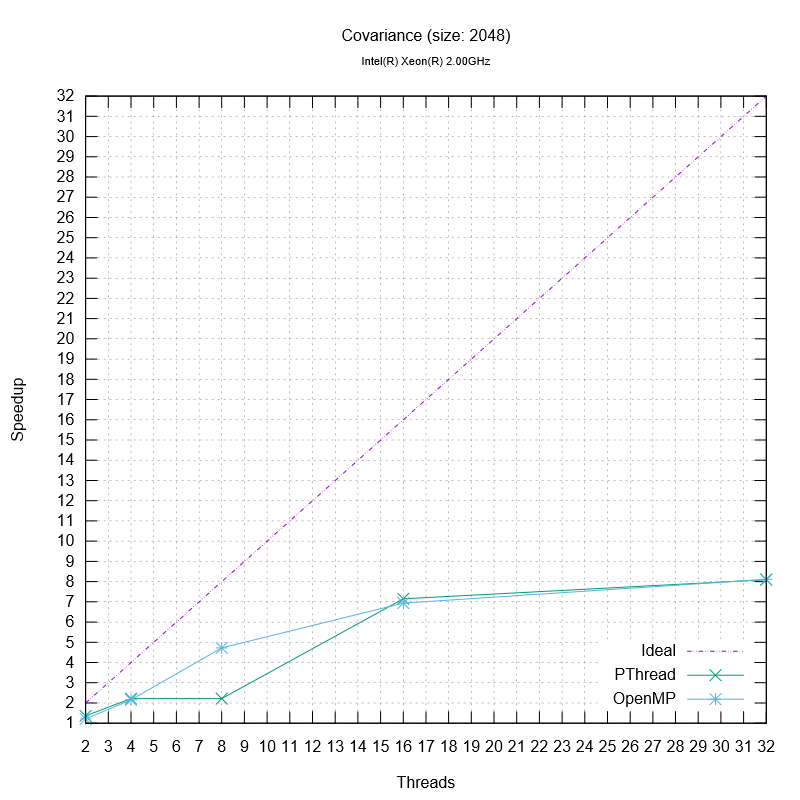
\includegraphics[width=1\textwidth]{speedup.png}
	\caption{Speedup do \textit{covariance}}
	\label{fig:speedup}
\end{figure}

Pode-se observar que não foi obtido um bom fator de aceleração, uma vez que as curvas da execução paralela ficaram bem distantes da curva ideal. Utilizar \textit{PThreads} se mostrou melhor para $2$, $4$ e $16$ \textit{threads}, enquanto o \textit{OpenMP} mostrou melhor tempo para $8$ \textit{threads}. Isso se deve ao fato de que as diretivas do \textit{OpenMP} implementam implicitamente barreiras. Para $32$ \textit{threads} já não se observa diferença e pode-se dizer que a partir desse valor, ambos algoritmos apresentariam resultados próximos.

Sobre a relação do programa com o \textit{hardware}, o sequencial apresentou número bem superiores em todos os contadores utilizados (\textit{cache miss} em L1, L2 e L3; instruções ponto flutuante; ciclos e instruções). Para o \textit{OpenMp}, as porcentagens dos números totais de cada contador com relação ao total do sequencial são: o número de L1 \textit{cache miss} representa $23,12\%$; o número de L2 \textit{cache miss} é $22,17\%$; L3 \textit{cache miss} $21,97\%$; são $22,44\%$ de instruções PF; $23,2\%$ de ciclos e $24,36\%$ de instruções. Ou seja, os valores para \textit{OpenMP} são por volta de 20\% dos valores sequenciais. Para as porcentagens do \textit{PThreads}, ocorrem valores próximos ao do \textit{OpenMP}. 

\section{Conclusões}

Como é possível observar na seção anterior (seção \ref{sec:resultados}), não foi obtido um bom \textit{speedup}. Diversos fatores poderiam ter contribuído para isso. A primeira delas seria o tamanho do problema. Foram realizados diversos testes para diversos tamanhos e, consequentemente, para diversos tempos, porém não houveram variações significativas do \textit{speedup}. Portanto, o tamanho do problema não foi o fator que provocou o baixo \textit{speedup}.

Um segundo fator seria excessos de \textit{cache miss}, como acontecem na execução sequencial. Todavia, em \textit{PThreads} e em \textit{OpenMP}, a quantidades de \textit{cache miss} são menores, equivalente a $20\%$ do sequencial. Sobre os resultados obtidos utilizando o PAPI, em resumo, mesmo que \textit{PThreads} e \textit{OpenMP} tenham contadores menores do que o sequencial para \textit{cache miss}, instruções de ponto flutuante, número de ciclos e de instruções, o \textit{speedup}, consideravelmente, bom não foi atingido (não foi atingido nem um \textit{speedup} $S\left(p\right)=10$ para $p \geq 10$).  

Portanto, pode-se afirmar que há dois possíveis fatores que, certamente, impactaram significativamente para o baixo fator de aceleração. O primeiro deles seria a necessidade de sincronização. Que possivelmente é a maior causa de \textit{overhead} nos tempos. A barreira necessária antes de um \textit{for} triplo pode ser o fator impactante para o baixo \textit{speedup}, ou o próprio \textit{for} triplo seja o fator impactante, ou ambos. E, por fim, a implementação ineficiente do código. Por exemplo, uso incorreto das diretivas do \textit{OpenMP} e/ou a divisão ineficiente de tarefas entre as \textit{threads} do \textit{PThread}.
 

\section{References}

\begin{itemize}
	\item Andrews, Gregory R. (1999)  \textit{Foundations of Multithreaded Parallel and Distributed Programming}. Editora Pearson, 1ª edição.
	\item Grama, Ananth; Karypis, George; Kumar, Vipin. (2003) \textit{Introduction to Parallel Computing}. Editora Pearson, 2ª edição.
    \item Mendes Jr., Pedro Ribeiro. (2012) Uso de paralelismo de dados em algoritmos de processamento de imagens utilizando Haskell. Monografia apresentada ao Curso de Bacharelado em Ciência da Computação da Universidade Federal de Ouro Preto, 52 páginas.
    \item Oliveira, Rebeka G. de; Cavalcante, Sérgio V. (2010) Explorando o paralelismo de dados e de thread para atingir a eficiência energética do ponto de vista do desenvolvedor de software. In anais da XXX Congresso da SBC, páginas 1776 -- 1789.
    \item \textit{OpenMP 4.5 Complete Specifications}. Disponível em <http://www.openmp.org/wp-content/uploads/openmp-4.5.pdf>, acesso em 24 de maio de 2017.
    \item Pacheco, Peter. (2011) \textit{An Introduction to Parallel Programming}. Editora Morgan Kaufmann, 1ª edição.
    \item Tutorial de \textit{POSIX Threads Programming}. In \textit{Lawrence Livermore National Laboratory}. Disponível em: <https://computing.llnl.gov/tutorials/pthreads/>, acesso em 24 de maio de 2017.
\end{itemize}

\bibliographystyle{sbc}

\end{document}
